\section{Language Server Protocol}\label{langserver}

Visual Studio Code plugins can be implemented in two ways: the first one is via the standard Visual Studio Code API and the second one is in form of a language server. Language servers follow a standard protocol to provide services for working with different programming languages and offer often used features such as go to definition. While this offers great portability and easy integration with other IDEs or tools that work with language servers, the implementation as a language server was at first rejected in this project. \newline
The main reason was that the project extends an existing plugin, which was already built around the standard Visual Studio Code API. A second consideration was that the usage of language servers in Visual Studio Code plugins is very sparse at the moment. The big language integrations like typescript or javascript do not implement their plugins as language servers, while the GoLang plugin offers experimental support at this time. The not wide spread usage in this environment was therefore another reason to not implement a language server initially. \newline
However, during the process of implementing the project, many features were faster done than initially estimated, and other planned features were proven to not be feasible for the scope of this work. This meant that more time could be spend on features or ideas that were labeled as optional in the beginning. Since the concept of a language server itself is intriguing due to the potential to widen the user base considerably, it was decided to try to restructure the plugin as a language server. \newline
The restructuring only took about 30 hours since the plugin was already nicely programmed in regard to separation of concerns, such that only a wrapper had to be written that implements the language server protocol and redirects the requests to the components that implement the core functionality. 
Since the plugin now is programmed in form of a language server, it can potentially easily be used in other IDEs such as Eclipse or Emacs once they fully implement the language server protocol on their side. In hindsight is thought that the change of the original decision and the additional work that had to be done was well worth regarding the resulting outcome. \newline

Below a short overview of the protocol and how it was implemented is given. Server here refers to the language server and not the DafnyServer. The later one is explicitly written as DafnyServer.

\subsection{The protocol}
The Language Server protocol is used between a tool (the client) and a language smartness provider (the server) to integrate features like auto complete, goto definition, find all references and alike into the tool. \cite{langserver} \newline

The language server maintains semantic information about a program implemented in a particular language. The language server is notified whenever the user opens a document in the tool. Also edits by the user are reported, so the language server is notified of the changes and can update the program's semantic information. Currently, only point to point communication is supported by the protocol. Sharing one language server between multiple tools would require further protocol mechanisms like locking a file.\newline
One of the most basic features is the analysis of the document and generation of errors and warnings (called diagnostics by Microsoft), which the tool then can display. Furthermore, more sophisticated features are also provided. For instance, the client can send a definition request for a symbol to the server. The server is then tasked to answer with the URI of the file and the range in that file where the definition can be found. The tool is then free to open said file or simply provide a peek at it through an overlay. \newline

\begin{figure}[H]
	\centering
	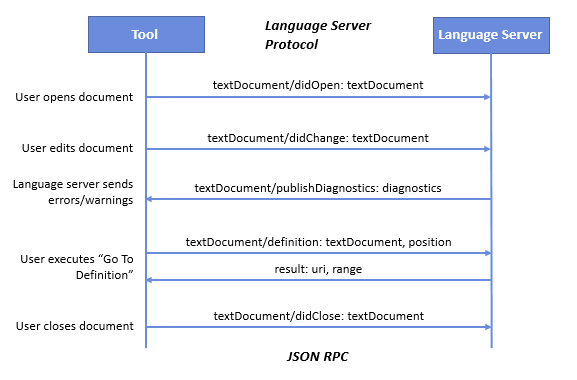
\includegraphics[width=1\textwidth]{img/langServerOverview}
	\caption{Example of the communication between the client and the server}
	\label{fig:langserveroverview}
\end{figure}


The server also gets notified when the user closes a file. An important distinction to make is that whenever the client has opened a file, it resides in memory and the tool maintains it. When it is closed, it simply lies in the file system like any other file. \newline
The communication between the tool and the language server uses JSON RPC v2.0. Language server can implement an arbitrary subset of features defined in the protocol, so in the first response by the server it details what capabilities it has. \newline


\subsection{Communication Types}
There are two different types to communicate between the client and the server. It's either a notification or a request. 

\paragraph{Notification}
A notification is just a message which can be sent in both directions. But one can't wait for an answer. These types of messages are mostly used to inform the partner that something happened. 

\paragraph{Request}
A request on the other side is a message which will be answered.  

\subsection{Standard Implementation}
Next to custom commands, which are explained in chapter \ref{custom commands} and following, the language server describes a standardized API\cite{protMaster} for features that are useful when working with a language server. The API is designed as a Request / Reply Protocol. Below a list of the implemented Requests is listed, while a detailed description on how the implementation was done can be found in \ref{architecture}. All the structures detailed in this chapter are defined by the protocol. \newline

\paragraph{Message Structure}
The protocol describes how the messages exchanged between the client and the server must be structured. A generic example of a request and a response are as follows:

\textbf{Request}
\begin{lstlisting}[language=json,firstnumber=1]
interface RequestMessage extends Message {

  /**
  * The request id.
  */
  id: number | string;

  /**
  * The method to be invoked.
  */
  method: string;

  /**
  * The method's params.
  */
  params?: any
}
\end{lstlisting}

\textbf{Response}
\begin{lstlisting}[language=json,firstnumber=1]
interface ResponseMessage extends Message {
  /**
  * The request id.
  */
  id: number | string | null;

  /**
  * The result of a request. This can be omitted in
  * the case of an error.
  */
  result?: any;

  /**
  * The error object in case a request fails.
  */
  error?: ResponseError<any>;
}

interface ResponseError<D> {
  /**
  * A number indicating the error type that occurred.
  */
  code: number;

  /**
  * A string providing a short description of the error.
  */
  message: string;

  /**
  * A Primitive or Structured value that contains additional
  * information about the error. Can be omitted.
  */
  data?: D;
}

export namespace ErrorCodes {
  // Defined by JSON RPC
  export const ParseError: number = -32700;
  export const InvalidRequest: number = -32600;
  export const MethodNotFound: number = -32601;
  export const InvalidParams: number = -32602;
  export const InternalError: number = -32603;
  export const serverErrorStart: number = -32099;
  export const serverErrorEnd: number = -32000;
  export const ServerNotInitialized: number = -32002;
  export const UnknownErrorCode: number = -32001;

  // Defined by the protocol.
  export const RequestCancelled: number = -32800;
}
\end{lstlisting}
\paragraph{Data structures}
Next, an overview over the most commonly used data structures used in the protocol is given: \newline

\textbf{Position}
Describes a position, e.g. of a cursor, in a document.
\begin{lstlisting}[language=json,firstnumber=1]
interface Position {
  /**
  * Line position in a document (zero-based).
  */
  line: number;

  /**
  * Character offset on a line in a document (zero-based).
  */
  character: number;
}
\end{lstlisting}

\textbf{Range}
Describes an area in a document which can span multiple lines of text.
\begin{lstlisting}[language=json,firstnumber=1]
interface Range {
  /**
  * The range's start position.
  */
  start: Position;

  /**
  * The range's end position.
  */
  end: Position;
}
\end{lstlisting}

\textbf{Location}
Describes a location inside a resource, such as a line inside a text file.
\begin{lstlisting}[language=json,firstnumber=1]
interface Location {
  uri: DocumentUri;
  range: Range;
}
\end{lstlisting}

\textbf{Diagnostic}
Describes a diagnostic such as an error or a compiler warning.
\begin{lstlisting}[language=json,firstnumber=1]
interface Diagnostic {
  /**
  * The range at which the message applies.
  */
  range: Range;

  /**
  * The diagnostic's severity. Can be omitted. If omitted it is up to the
  * client to interpret diagnostics as error, warning, info or hint.
  */
  severity?: number;

  /**
  * The diagnostic's code. Can be omitted.
  */
  code?: number | string;

  /**
  * A human-readable string describing the source of this
  * diagnostic, e.g. 'typescript' or 'super lint'.
  */
  source?: string;

  /**
  * The diagnostic's message.
  */
  message: string;
}
\end{lstlisting}

\textbf{Server capabilities}
With this data structure, the server can tell the client which features it implements. 
\begin{lstlisting}[language=json,firstnumber=1]
interface ServerCapabilities {
  /**
  * Defines how text documents are synced. Is either a detailed structure defining each notification or
  * for backwards compatibility the TextDocumentSyncKind number.
  */
  textDocumentSync?: TextDocumentSyncOptions | number;
  /**
  * The server provides hover support.
  */
  hoverProvider?: boolean;
  /**
  * The server provides completion support.
  */
  completionProvider?: CompletionOptions;
  /**
  * The server provides signature help support.
  */
  signatureHelpProvider?: SignatureHelpOptions;
  /**
  * The server provides goto definition support.
  */
  definitionProvider?: boolean;
  /**
  * The server provides find references support.
  */
  referencesProvider?: boolean;
  /**
  * The server provides document highlight support.
  */
  documentHighlightProvider?: boolean;
  /**
  * The server provides document symbol support.
  */
  documentSymbolProvider?: boolean;
  /**
  * The server provides workspace symbol support.
  */
  workspaceSymbolProvider?: boolean;
  /**
  * The server provides code actions.
  */
  codeActionProvider?: boolean;
  /**
  * The server provides code lens.
  */
  codeLensProvider?: CodeLensOptions;
  /**
  * The server provides document formatting.
  */
  documentFormattingProvider?: boolean;
  /**
  * The server provides document range formatting.
  */
  documentRangeFormattingProvider?: boolean;
  /**
  * The server provides document formatting on typing.
  */
  documentOnTypeFormattingProvider?: DocumentOnTypeFormattingOptions;
  /**
  * The server provides rename support.
  */
  renameProvider?: boolean;
  /**
  * The server provides document link support.
  */
  documentLinkProvider?: DocumentLinkOptions;
  /**
  * The server provides execute command support.
  */
  executeCommandProvider?: ExecuteCommandOptions;
  /**
  * Experimental server capabilities.
  */
  experimental?: any;
}
\end{lstlisting}

\paragraph{Implemented Requests}
Next, pairs of Request / Responses implemented by this project are listed:

\textbf{Shutdown Request}

The shutdown request is sent from the client to the server. It asks the server to shut down, but to not exit (otherwise the response might not be delivered correctly to the client). There is a separate exit notification that asks the server to exit.

Request:
\begin{lstlisting}[language=json,firstnumber=1]
  method: 'shutdown'
  params: void
\end{lstlisting}
Response:
\begin{lstlisting}[language=json,firstnumber=1]
result: null
error: code and message set in case an exception happens during shutdown request.
\end{lstlisting}

\textbf{Exit Notification}

A notification to ask the server to exit its process. The server should exit with success code 0 if the shutdown request has been received before; otherwise with error code 1.

Notification:
\begin{lstlisting}[language=json,firstnumber=1]
method: 'exit'
params: void
\end{lstlisting}

\textbf{ShowMessage Notification}

The show message notification is sent from a server to a client to ask the client to display a particular message in the user interface.

Notification:
\begin{lstlisting}[language=json,firstnumber=1]
method: 'window/showMessage'
params: ShowMessageParams defined as follows:
interface ShowMessageParams {
  /**
  * The message type. See {@link MessageType}.
  */
  type: number;
	
  /**
  * The actual message.
  */
  message: string;
}
\end{lstlisting}
\textbf{ShowMessage Request}

The show message request is sent from a server to a client to ask the client to display a particular message in the user interface. In addition to the show message notification the request allows to pass actions and to wait for an answer from the client.

Request:
\begin{lstlisting}[language=json,firstnumber=1]
method: 'window/showMessageRequest'
params: ShowMessageRequestParams
\end{lstlisting}
Response:
\begin{lstlisting}[language=json,firstnumber=1]
result: the selected MessageActionItem
error: code and message set in case an exception happens during showing a message.
interface ShowMessageRequestParams {
  /**
  * The message type. See {@link MessageType}
  */
  type: number;
	
  /**
  * The actual message
  */
  message: string;
	
  /**
  * The message action items to present.
  */
  actions?: MessageActionItem[];
}
\end{lstlisting}

\textbf{DidChangeConfiguration Notification}

A notification sent from the client to the server to signal the change of configuration settings.

Notification:
\begin{lstlisting}[language=json,firstnumber=1]
method: 'workspace/didChangeConfiguration',
params: DidChangeConfigurationParams defined as follows:
interface DidChangeConfigurationParams {
  /**
  * The actual changed settings
  */
  settings: any;
}
\end{lstlisting}

\textbf{DidOpenTextDocument Notification}

The document open notification is sent from the client to the server to signal newly opened text documents. The document's truth is now managed by the client and the server must not try to read the document's truth using the document's Uri.

Notification:
\begin{lstlisting}[language=json,firstnumber=1]
method: 'textDocument/didOpen'
params: DidOpenTextDocumentParams defined as follows:
interface DidOpenTextDocumentParams {
  /**
  * The document that was opened.
  */
  textDocument: TextDocumentItem;
}
\end{lstlisting}

\textbf{DidChangeTextDocument Notification}

The document change notification is sent from the client to the server to signal changes to a text document. In 2.0 the shape of the params has changed to include proper version numbers and language ids.

Notification:
\begin{lstlisting}[language=json,firstnumber=1]
method: 'textDocument/didChange'
params: DidChangeTextDocumentParams defined as follows:
interface DidChangeTextDocumentParams {
  /**
  * The document that did change. The version number points
  * to the version after all provided content changes have
  * been applied.
  */
  textDocument: VersionedTextDocumentIdentifier;
	
  /**
  * The actual content changes.
  */
  contentChanges: TextDocumentContentChangeEvent[];
}
\end{lstlisting}

\textbf{DidCloseTextDocument Notification}

The document close notification is sent from the client to the server when the document got closed in the client. The document's truth now exists where the document's Uri points to (e.g. if the document's Uri is a file Uri the truth now exists on disk).

Notification:
\begin{lstlisting}[language=json,firstnumber=1]
method: 'textDocument/didClose'
params: DidCloseTextDocumentParams defined as follows:
interface DidCloseTextDocumentParams {
  /**
  * The document that was closed.
  */
  textDocument: TextDocumentIdentifier;
}
\end{lstlisting}

\textbf{PublishDiagnostics Notification}

Diagnostics notification are sent from the server to the client to signal results of validation runs.

Notification:
\begin{lstlisting}[language=json,firstnumber=1]
method: 'textDocument/publishDiagnostics'
params: PublishDiagnosticsParams defined as follows:
interface PublishDiagnosticsParams {
  /**
  * The URI for which diagnostic information is reported.
  */
  uri: DocumentUri;
	
  /**
  * An array of diagnostic information items.
  */
  diagnostics: Diagnostic[];
}
\end{lstlisting}
\textbf{Completion Request}

The Completion request is sent from the client to the server to compute completion items at a given cursor position. Completion items are presented in the IntelliSense user interface. If computing full completion items is expensive, servers can additionally provide a handler for the completion item resolve request ('completionItem/resolve'). This request is sent when a completion item is selected in the user interface. A typically use case is for example: the 'textDocument/completion' request doesn't fill in the documentation property for returned completion items since it is expensive to compute. When the item is selected in the user interface then a 'completionItem/resolve' request is sent with the selected completion item as a param. The returned completion item should have the documentation property filled in.

Request:
\begin{lstlisting}[language=json,firstnumber=1]
method: 'textDocument/completion'
params: TextDocumentPositionParams
\end{lstlisting}
Response:
\begin{lstlisting}[language=json,firstnumber=1]
result: CompletionItem[] | CompletionList
/**
* Represents a collection of [completion items](#CompletionItem) to be presented
* in the editor.
*/
interface CompletionList {
  /**
  * This list it not complete. Further typing should result in recomputing
  * this list.
  */
  isIncomplete: boolean;
  /**
  * The completion items.
  */
  items: CompletionItem[];
}
\end{lstlisting}

\textbf{Goto Definition Request}

The goto definition request is sent from the client to the server to resolve the definition location of a symbol at a given text document position.

Request:
\begin{lstlisting}[language=json,firstnumber=1]
method: 'textDocument/definition'
params: TextDocumentPositionParams
\end{lstlisting}

Response:
\begin{lstlisting}[language=json,firstnumber=1]
result: Location | Location[]
error: code and message set in case an exception happens during the definition request.
Registration Options: TextDocumentRegistrationOptions
\end{lstlisting}

\textbf{Find References Request}

The references request is sent from the client to the server to resolve project-wide references for the symbol denoted by the given text document position.

Request:
\begin{lstlisting}[language=json,firstnumber=1]
method: 'textDocument/references'
params: ReferenceParams defined as follows:
interface ReferenceParams extends TextDocumentPositionParams {
	context: ReferenceContext
}
interface ReferenceContext {
  /**
  * Include the declaration of the current symbol.
  */
  includeDeclaration: boolean;
}
\end{lstlisting}
Response:
\begin{lstlisting}[language=json,firstnumber=1]
result: Location[]
error: code and message set in case an exception happens during the reference request.
Registration Options: TextDocumentRegistrationOptions
\end{lstlisting}

\textbf{Code Action Request}

The code action request is sent from the client to the server to compute commands for a given text document and range. These commands are typically code fixes to either fix problems or to beautify/refactor code.

Request:
\begin{lstlisting}[language=json,firstnumber=1]
method: 'textDocument/codeAction'
params: CodeActionParams defined as follows:
/**
* Params for the CodeActionRequest
*/
interface CodeActionParams {
  /**
  * The document in which the command was invoked.
  */
  textDocument: TextDocumentIdentifier;
	
  /**
  * The range for which the command was invoked.
  */
  range: Range;
	
  /**
  * Context carrying additional information.
  */
  context: CodeActionContext;
}

/**
* Contains additional diagnostic information about the context in which
* a code action is run.
*/
interface CodeActionContext {
  /**
  * An array of diagnostics.
  */
  diagnostics: Diagnostic[];
}
\end{lstlisting}
Response:
\begin{lstlisting}[language=json,firstnumber=1]
result: Command[] defined as follows:
error: code and message set in case an exception happens during the code action request.
Registration Options: TextDocumentRegistrationOptions
\end{lstlisting}

\textbf{Code Lens Request}

The code lens request is sent from the client to the server to compute code lenses for a given text document.

Request:
\begin{lstlisting}[language=json,firstnumber=1]
method: 'textDocument/codeLens'
params: CodeLensParams defined as follows:
interface CodeLensParams {
  /**
  * The document to request code lens for.
  */
  textDocument: TextDocumentIdentifier;
}
\end{lstlisting}
Response:
\begin{lstlisting}[language=json,firstnumber=1]
result: CodeLens[] defined as follows:
/**
* A code lens represents a command that should be shown along with
* source text, like the number of references, a way to run tests, etc.
*
* A code lens is _unresolved_ when no command is associated to it. For performance
* reasons the creation of a code lens and resolving should be done in two stages.
*/
interface CodeLens {
  /**
  * The range in which this code lens is valid. Should only span a single line.
  */
  range: Range;
	
  /**
  * The command this code lens represents.
  */
  command?: Command;
	
  /**
  * A data entry field that is preserved on a code lens item between
  * a code lens and a code lens resolve request.
  */
  data?: any
}
error: code and message set in case an exception happens during the code lens request.
\end{lstlisting}

\textbf{Code Lens Resolve Request}

The code lens resolve request is sent from the client to the server to resolve the command for a given code lens item.

Request:
\begin{lstlisting}[language=json,firstnumber=1]
method: 'codeLens/resolve'
params: CodeLens
\end{lstlisting}

Response:
\begin{lstlisting}[language=json,firstnumber=1]
result: CodeLens
error: code and message set in case an exception happens during the code lens resolve request.
\end{lstlisting}

\textbf{Rename Request}

The rename request is sent from the client to the server to perform a workspace-wide rename of a symbol.

Request:
\begin{lstlisting}[language=json,firstnumber=1]
method: 'textDocument/rename'
params: RenameParams defined as follows
interface RenameParams {
  /**
  * The document to format.
  */
  textDocument: TextDocumentIdentifier;

  /**
  * The position at which this request was sent.
  */
  position: Position;

  /**
  * The new name of the symbol. If the given name is not valid the
  * request must return a [ResponseError](#ResponseError) with an
  * appropriate message set.
  */
  newName: string;
}
\end{lstlisting}
Response:
\begin{lstlisting}[language=json,firstnumber=1]
result: WorkspaceEdit describing the modification to the workspace.
error: code and message set in case an exception happens during the rename request.
Registration Options: TextDocumentRegistrationOptions
\end{lstlisting}

\subsection{Communication overview}\label{custom commands}
All the following notifications and requests are not standadized. They were needed to have additional features like installing Dafny, restarting the DafnyServer or updating the queue size. 
Therefore to support a new IDE all the \textbf{Server $\longrightarrow$ Client} have to be implemented, in the new client.

\subsubsection{Notification Server $\longrightarrow$ Client}

\textbf{ERROR}
This message is sent if something happens which the user should be informed about. Examples would be that the compilation failed or the DafnyServer wasn't found. \newline

\textbf{WARNING}
This message is sent if the mono path is specified but mono is in the path. \newline

\textbf{INFO}
Info messages appear quite often to inform the user about the current progress. \newline

\textbf{dafnymissing}
This informs the client that the verification of the DafnyServer has failed or that there is a newer version available. The text is sent as a additional parameter.  \newline

\textbf{queueSize}
This message updates the queue size number in the status bar on the right side. \newline

\textbf{serverStarted}
This message contains two additional parameters, which are also important for the status bar. They are the PID and the version of the started DafnyServer instance. It is sent after the dependencies have been checked and the DafnyServer have been spawned. \newline

\textbf{activeVerifiyingDocument}
As soon as a verification is sent to the DafnyServer, the client is informed to show that, if the user has this file open. \newline

\textbf{verificationResult}
All verification results are sent to the server, for fast access times. Switching from one file to the other, updates the verification result on the left side based on these results. \newline

\textbf{changeServerStatus}
All states from the server are also sent to the client to update the status bar. \newline

\textbf{ready}
This message is sent directly after the serverStarted message to inform the DafnyClientProvider that verification requests can now be sent. \newline

\textbf{progress}
Used for inform user about progress during downloading and extracting of Dafny. This notification has also the following data attached: domain, current, total\newline

\subsubsection{Request Server $\longrightarrow$ Client}
There are no requests which are sent from the server. 


\subsubsection{Diagnostics Server $\longrightarrow$ Client}

\textbf{sendDiagnostics}
After a file has been verified, the output is analyzed and errors are sent as diagnostics to the client. They contain also the message or even related locations, where the errors is coming from.  \newline

\subsubsection{Notification Client $\longrightarrow$ Server}

\textbf{verify}
This notification contains the document which has to be verified. On the server it is put into a queue and the result is sent via verificationResult. \newline

\textbf{counterExample}
This message is sent directly after the serverStarted message to inform the DafnyClientProvider that verification requests can now be sent. \newline


\subsubsection{Request Client $\longrightarrow$ Server}

\textbf{reset}
Resets the DafnyServer on the Server and restarts it. This can be useful if the caching of the DafnyServer is not working correctly anymore. \newline

\textbf{compile}
Sends a request containing only the Uri to the corresponding file. Starts the Dafny.exe with parameters to generate either a dll or an exe. After the compilation, it returns possible errors, if it is executable and a message.\newline

\textbf{install}
Executes first an uninstallation if Dafny is installed. Afterwards downloads Dafny, extracts it. Additionally the install folder is sent in the response to update the configuration. \newline

\textbf{uninstall}
First stops the running instance and then removes the current Dafny installation. \newline

\textbf{dotgraph}
Generates a flowgraph for the file sent. Returns as the generation has been completed. \newline

\subsection{Commands}
Commands are specified in the client and can trigger different actions. One can specify names for them and register shortcuts from them. The server can also send commands. This was needed for example, to show references, because there was a transform necessary, so that the arguments are the right types, before the command is executed. The method signature was not the same as in the language server protocol specification. 

\subsubsection{Commands Server}
\textbf{dafny.showReferences}
Used by CodeLens to show references of methods. The method transforms the arguments and forward them to the \textbf{editor.action.showReferences} command. 

\textbf{dafny.editText}
Used by rename to do text modifications. Should process all text edits which are sent. 

\subsubsection{Commands Client}

\textbf{dafny.restartDafnyServer}
Restarts the DafnyServer with the "Reset Request".\newline

\textbf{dafny.installDafny}
This command is used to trigger the install request, either by a context menu or a shortcut. 
First run the uninstallDafny command to be sure that there is no running instance. Afterwards downloads the latest version from GitHub. This process is either executed from an upgrade message, not installed message or can be executed manually. 
See \nameref{fig:Version upgrade available} for a better overview over the installation process. \newline

\textbf{dafny.uninstallDafny}
First stops any DafnyServer instance and deletes all files which belongs to Dafny. \newline

\textbf{dafny.showReferences}
This is used to show references from CodeLenses. Unfortunately the command editor.action.showReferences can not be used directly, because of some internal problems. To solve that, all parameters have to be copied and passed to this command. \newline

\textbf{dafny.editText}
Mainly used for all refactoring to change text in the active text document. \newline

\textbf{dafny.compile}
\todo{add mac shortcut correctly}
Shortcut: ctrl+shift+b or %⇧⌘B 
\newline
Compile the current document \newline

\textbf{dafny.compileAndRun}
Shortcut: F5
\newline
Compile the current document, and if there is a "Main Method", start the corresponding executable. \newline

\textbf{dafny.showCounterExample}
Shortcut: F7
\newline
Calculates the counter example for the current file. \newline


\textbf{dafny.hideCounterExample}
Shortcut: F8
\newline
Hide the counter example in the current file.  \newline

\textbf{dafny.showDotGraph}
Shortcut: F6
\newline
Generates a flow graph out of the current file. Displays all the graphs in a second view. \newline


\subsection{Process overview}
\subsubsection{Startup process}
\begin{figure}[H]
	\centering
	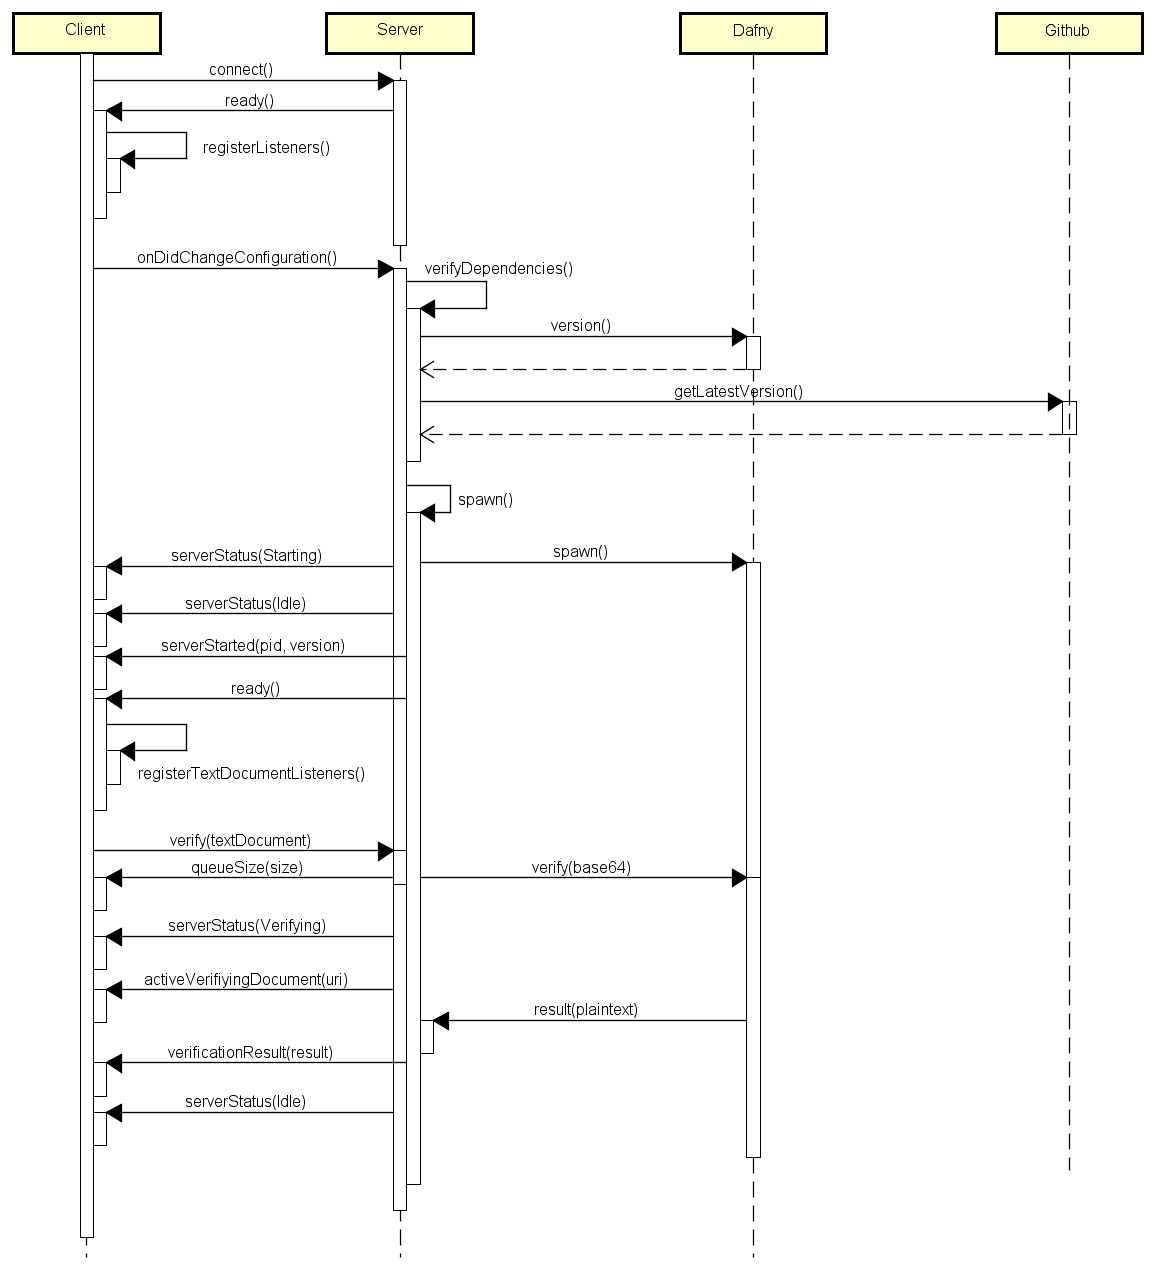
\includegraphics[width=1\textwidth]{img/DafnyStartupFull}
	\caption{DafnyServer startup}
	\label{fig:DafnyServer startup}
\end{figure}

\subsubsection{Not installed}
\begin{figure}[H]
	\centering
	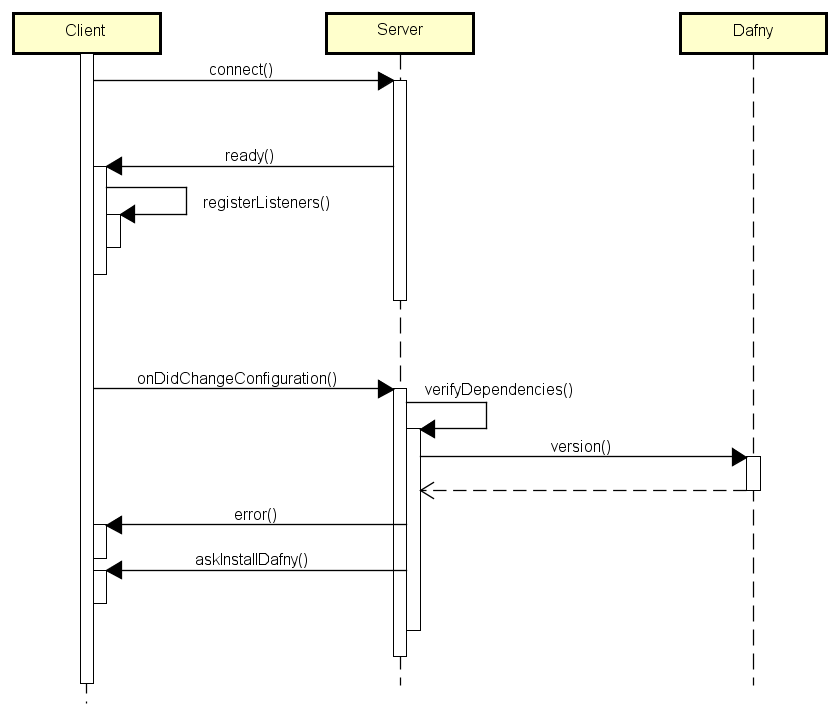
\includegraphics[width=1\textwidth]{img/DafnyNotInstalled}
	\caption{Dafny not installed}
	\label{fig:Dafny not installed}
\end{figure}

\subsubsection{Installation - Upgrade available}
\begin{figure}[H]
	\centering
	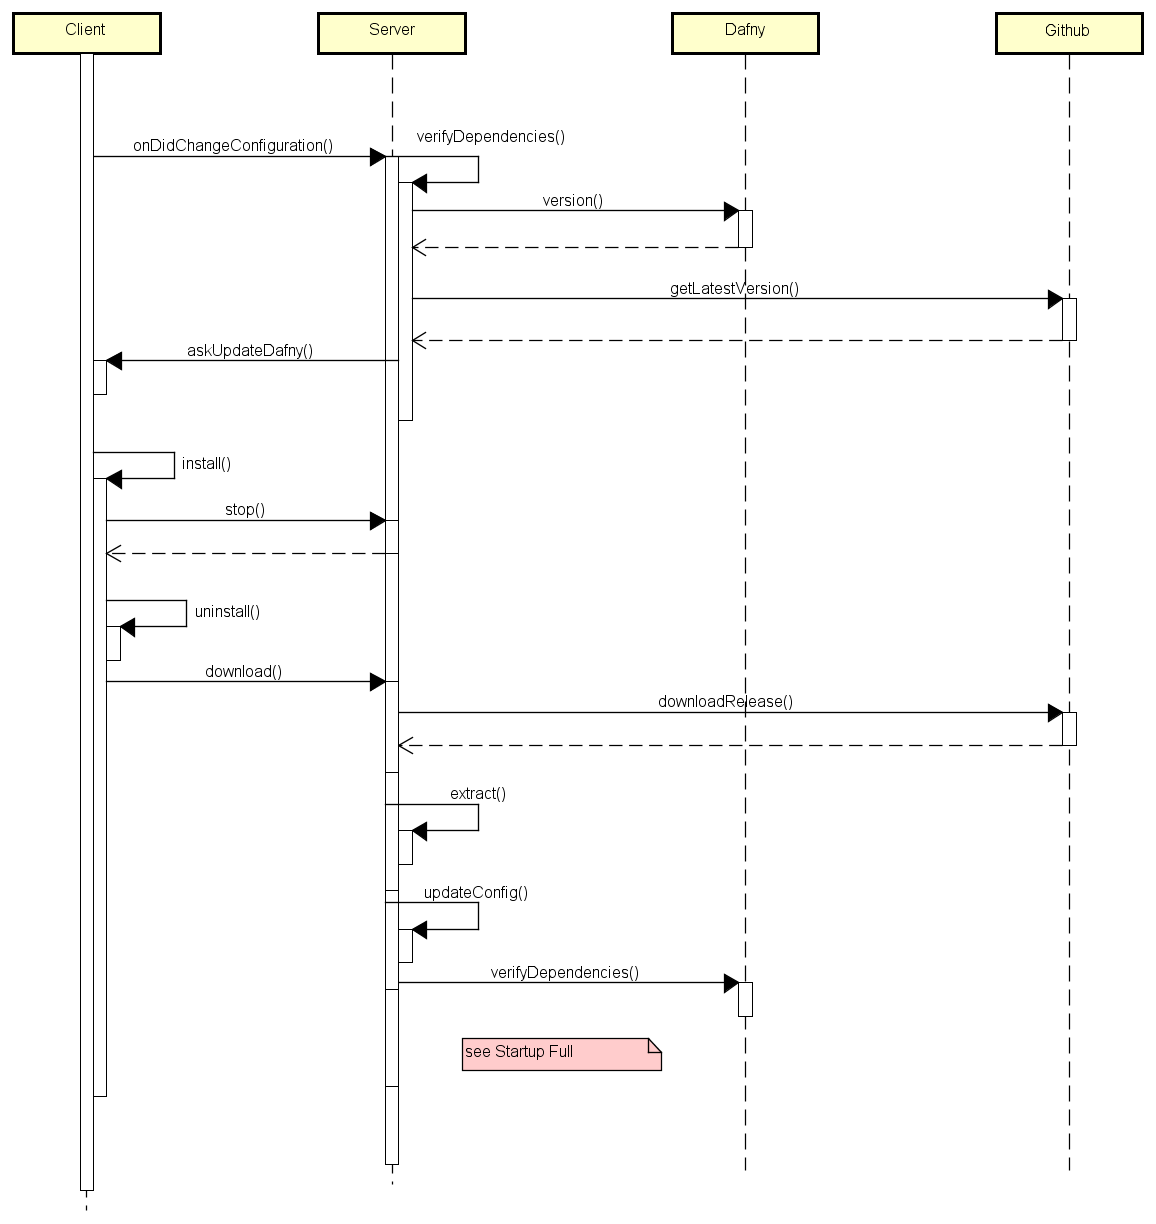
\includegraphics[width=1\textwidth]{img/DafnyVersionUpgrade}
	\caption{Version upgrade available}
	\label{fig:Version upgrade available}
\end{figure}



